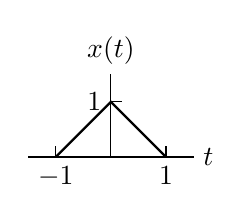
\begin{tikzpicture}[scale=0.70]
	\begin{scope}
		\draw (-1.5,0) -- (1.5,0) node[anchor=west] {$t$};
		\draw (0, 0) -- (0,1.5) node[anchor=south] {$x(t)$};	
		\foreach \x in {-1, 1}
		{
			\draw (\x, 0.2) -- ++(0, -0.2);
			\node at (\x, 0) [anchor=north ] {$\x$};
		}
		\foreach \y in {1}
		{
			\draw (0.2, \y) -- ++(-0.2, 0);
			\node at (0, \y) [anchor=east ] {$\y$};
		}	
		
		\draw[thick] (-1,0) -- (0,1) -- (1,0); 
	\end{scope}
	
\end{tikzpicture} 